\documentclass[11pt, a4paper]{article} % setsfont size and layout

%% required packages %%

\usepackage[margin=2.5cm]{geometry} % margins
\usepackage[utf8]{inputenc} % Umlaute
\usepackage{amsmath,amssymb, physics}		% math formulas
\usepackage{graphicx}		% graphics
\usepackage{fancyhdr}		% header and footer on every page
\usepackage{setspace}		% line space (e.g. \singlespacing, \onehalfspacing or \doublespacing)

\usepackage{braket}
\usepackage{xcolor}
%% Here the main part of the document begins %%

\begin{document}
	
%% Some more settings %%
	
\setlength{\parindent}{0pt} % first line in paragraph will not be indented
\onehalfspacing				% 1.5 line spacing
%\thispagestyle{empty}		% no header and page number on first page


%% Header on first page with course information etc. %%
%\begin{tabular}{p{15.5cm}}
%	{\large \textbf{Classical Mechanics}} \\
%	Westlake University \\ 
%	\hline
%	\\
%\end{tabular}

\vspace*{0.1cm}				% vertical space between header on top of the page and main heading


\begin{center}
	{\Large \textbf{Classical Mechanics}}
    \vspace*{2mm}
    
    {\Large \textbf{Final Exam}}
	\vspace{8mm}
%Name: 
%\end{center} 
%\vspace{0.1cm}

{\Large \bf \color{red} Time: 2:00 - 4:00 pm, Dec. 30th, 2025}
\vspace*{2mm}

{\Large \bf \color{red} Duration: 120 minutes}
\vspace*{2mm}

{\Large \bf \color{red} Total Points: 100 out of 110}
\end{center}
\vspace*{8mm}

{\Large \bf \color{orange} Instruction:} 
\vspace*{2mm}

{\Large \bf \color{orange} \hspace{2em} This is a closed-book exam; no aids are allowed.}
\vspace*{2mm}

{\Large \bf \color{orange} \hspace{2em} Total 11 pages including the front page of the instruction.}
\vspace*{2mm}

{\Large \bf \color{orange} \hspace{2em} Provide relevant mathematical steps.} 
\vspace*{2mm}

{\Large \bf \color{orange} \hspace{2em} All answers must be in English.}
\vspace*{2mm}

{\Large \bf \color{orange} \hspace{2em} Don't open the booklet before the exam begins.}
\vspace{5cm}

\begin{center}
{\Large \bf Student Name: \underline{\hbox to 40mm{}}}
\vspace*{8mm}

{\Large \bf Student ID: \underline{\hbox to 40mm{}}}
\vspace*{2mm}
\end{center}

\newpage
\section*{Problem 1 [$5 + 5$ points]} 
\begin{enumerate}
  \item[(1)] Write down Newton’s second law, the Euler-Lagrange equation, and Hamilton’s equations of motion. 

  \item[(2)] State the principle of virtual work for a mechanical system in static equilibrium. Starting from Newton’s second law, derive the principle of virtual work.

  \end{enumerate}


\newpage 
\section*{Problem 2 [$4+3+3$ points]} 
Let the Lagrangian of a system be given by $L(q_k, \dot{q}_k, t)$, where $q_k$ and $\dot{q}_k$ denote the generalized coordinates and velocities, respectively, for $k = 1, \dots, n$. 
The Hamiltonian function is then defined as
\[
H(q_k, p_k, t) = \sum_{k=1}^n p_k \dot{q}_k - L(q_k, \dot{q}_k, t),
\]
where the velocities $\dot{q}_k$ are to be considered as functions of $(q_k, p_k, t)$, implicitly defined via the Legendre transformation.

\begin{enumerate}
  \item[(1)] Compute the total differential $\dd H$ of the Hamiltonian. Express your result in terms of the differentials $\dd q_k$, $\dd p_k$, $\dd\dot{q}_k$, and $\dd t$. 
  
  \item[(2)] Using the result of (1), derive Hamilton's equations of motion.
  
  \item[(3)] Prove that if the Lagrangian $L(q_k, \dot{q}_k)$ does not depend explicitly on time $t$, then the Hamiltonian $H$ is conserved.

\end{enumerate}

\newpage
\section*{Problem 3 [$10$ points]}
A bead of mass $m$ slides on a frictionless rod inclined at a constant angle $\alpha$ to the vertical axis. The rod rotates about this vertical axis with a constant angular velocity $\omega$. Gravity $g$ acts vertically downwards. Derive the equation of motion for the position $r$ of the bead along the rod using the Lagrangian formalism. 
\begin{figure}[h]
    \centering
    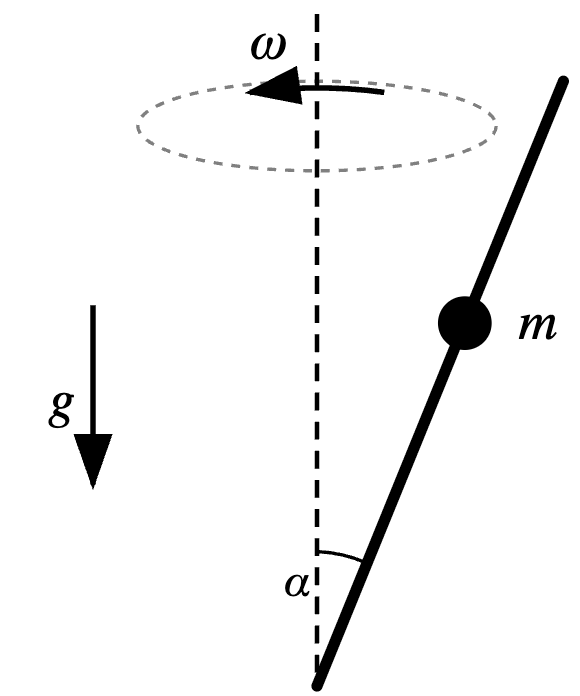
\includegraphics[width=0.35\textwidth]{bead.png}
    \label{P7}
\end{figure}

\newpage
\section*{Problem 4 [$10$ points]}
A block of mass $m$ is held motionless on a frictionless plane of mass $M$ and angle of inclination $\theta$ (see the Figure below). The plane rests on a frictionless horizontal surface. The block is released. What is the horizontal acceleration of the plane of mass $M$?

\begin{figure}[h]
    \centering
    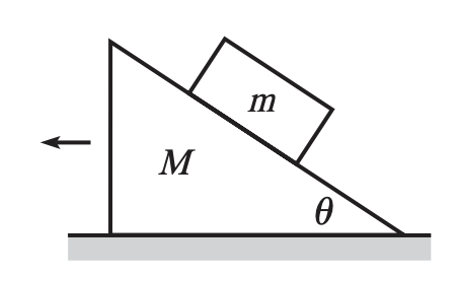
\includegraphics[width=0.4\textwidth]{Finala_P7.png}
    \label{P7}
\end{figure}

\newpage
\section*{Problem 5 [$5+5$ points]}
A system with one degree of freedom has Hamiltonian 
\begin{equation*}
    H(q,p) = \frac{p^2}{2m} + A(q)p + B(q)
\end{equation*}
where $A$ and $B$ are certain functions of the coordinate $q$, and $p$ is the momentum.

\begin{enumerate}
\item[(1)] Find the generalized velocity $\dot{q}$.

\item[(2)]  Find the Lagrangian $L(q, \dot{q})$.
\end{enumerate}

\newpage
\section*{Problem 6 [$10$ points]}
Consider a one-dimensional harmonic oscillator with Hamiltonian:
\begin{equation*}
    H(q, p) = \frac{1}{2}\left(p^2 + \omega^2 q^2\right),
\end{equation*}
where $q$ and $p$ are the generalized coordinate and momentum, respectively, and $\omega$ is the angular frequency. Let the generating function of the canonical transformation be of type I (a function of the old coordinate $q$ and the new coordinate $Q$), given by:
\begin{equation*}
    F_1(q, Q) = \frac{1}{2} \omega q^2 \cot(2\pi Q).
\end{equation*}

\begin{enumerate}
    \item[(1)] Determine the new Hamiltonian $K(Q, P)$ by performing the canonical transformation defined by the generating function $F_1(q, Q)$. Hint: $p=\frac{\partial F_1}{\partial q}$ and $P=-\frac{\partial F_1}{\partial Q}$.

    \item[(2)] Express the time evolution of the original variables $q(t)$ and $p(t)$ in terms of the new canonical momentum $P$, the frequency $\omega$, and time $t$.
\end{enumerate}


\newpage
\section*{Problem 7 [$6+6$ points]}
A satellite of mass $m$ carrying a crew is initially in a stable circular orbit (Orbit 1) of radius $R_1$ around a central body of mass $M$. The crew wishes to transfer the satellite to a larger circular orbit (Orbit 3) with a radius of $R_3 = 2R_1$. To achieve this, they perform a maneuver involving two successive impulsive boosts. 
First, the satellite performs an initial boost that increases its velocity instantaneously, placing it onto an elliptical transfer orbit (denoted as Orbit 2). This transfer orbit has its perigee at radius $R_1$ (the radius of the initial circular orbit) and its apogee at $R_3 = 2R_1$.
Next, upon reaching the apogee of the transfer orbit (point $P'$), the satellite performs a second instantaneous velocity change. This second boost increases the satellite's speed such that it transitions into a final circular orbit of radius $2R_1$.
\begin{enumerate}
    \item[(1)] Determine the thrust factor $\lambda$ required for the first boost, defined as the ratio of the speed after the boost to the speed before the boost ($\lambda = v_{p} / v_1$).
    \item[(2)] Determine the thrust factor $\lambda'$ required for the second boost, defined as the ratio of the speed after the boost to the speed before the boost ($\lambda' = v_3 / v_{p'}$).
\end{enumerate}

\textbf{Hint:} The orbit of a satellite is given by $
r(\phi) = \frac{c}{1 + \epsilon \cos \phi}$. 
$\epsilon$ is the eccentricity of the orbit; $c = \frac{L^2}{GMm^2}$, where $L$ is the satellite’s angular momentum.

\begin{figure}[h]
    \centering
    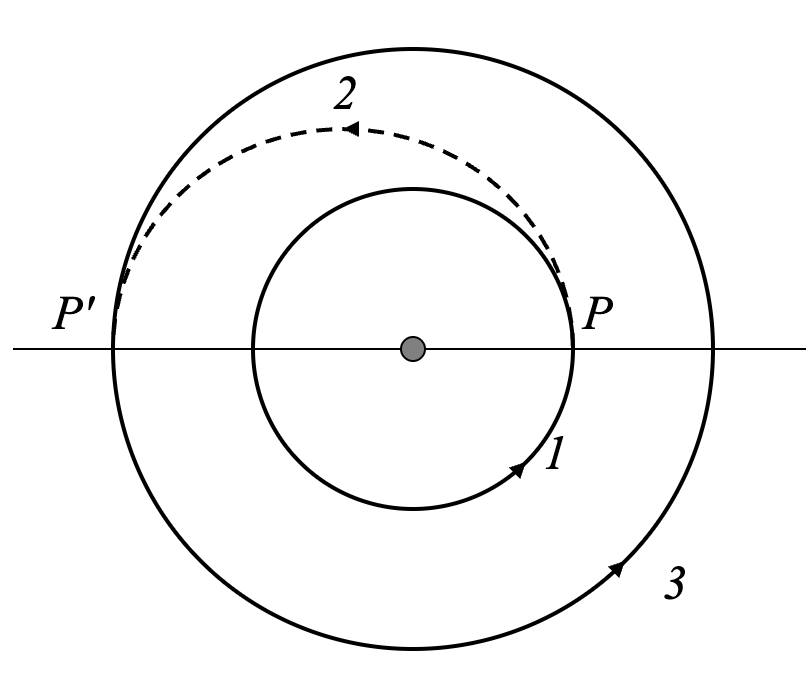
\includegraphics[width=0.3\textwidth]{transfer.png}
    \label{P7}
\end{figure}

% \newpage
% \section*{Problem 5 [$5+5$ points]}
% \begin{enumerate}
% \item[(1)] Prove that the transformation 
% \begin{equation*}
%    Q = p/\tan q
% \end{equation*}
% \begin{equation*}
% P = \ln{\left(\frac{\sin q}{p}\right)}
% \end{equation*}
% is canonical. 
% \item[(2)] Find the generating function $F_1(q, Q)$ for this transformation.
% \end{enumerate}

\newpage
\section*{Problem 8 [$6 + 10$ points]}
\begin{enumerate}
\item[(1)]  What are the conditions on the ``small" constants $a$, $b$, $c$, $d$, $e$, and $f$ in order that 
\begin{equation*}
    q= Q+ aQ^2+2bQP + cP^2
\end{equation*}
\begin{equation*}
   p=P+dQ^2+2eQP+fP^2
\end{equation*}
be canonical transformation to \textbf{first order} in small quantities?

\item[(2)] The Hamiltonian for a slightly anharmonic oscillator is 
\begin{equation*}
   H=\frac{p^2}{2m} + \frac{1}{2}m\omega^2q^2 + \beta q^3
\end{equation*}
where $\beta$ is ``small". Perform a canonical transformation of the type given in (1) and adjust the constants so that the new Hamiltonian $H$ does not contain an anharmonic term to first order in small quantities, thus 
\begin{equation*}
   H'=\frac{P^2}{2m} + \frac{1}{2}m\omega^2Q^2 + ...
\end{equation*}
Write down the transformations rules between $(q, p)$ and $(Q, P)$.
\end{enumerate}

% \newpage
% \section*{Problem 8 [10 points]}
% \hspace{2em} A Hamiltonian with one degree of freedom has the form
% \begin{equation*}
%     H = \frac{p^2}{2m} + \frac{kq^2}{2} - 2aq^3\sin\alpha t
% \end{equation*}
% where $m$, $k$, $a$, and $\alpha$ are constants. Find the Lagrangian corresponding to this Hamiltonian. Write out both Hamilton's equations and Euler-Lagrange equations, and show directly that they are equivalent.
% \end{enumerate}


\newpage
\section*{Problem 9 [$12$ points ]}
A pendulum consists of a mass $m$ at the end of a massless stick of length $l$. The other end of the stick is made to oscillate vertically with a position given by $y(t) = A \cos(\omega t)$, where $A \ll l$. It turns out that if $\omega$ is large enough, and if the pendulum is initially nearly upside-down, then surprisingly it will not fall over as time goes by. Find the equation of motion for the angle of the pendulum (measured relative to its upside-down position). You may simply the final equation of motion using the small-angle approximation.

\begin{figure}[h]
    \centering
    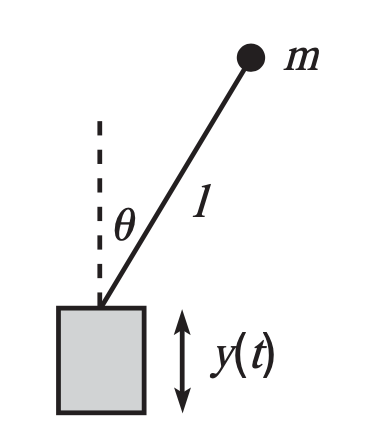
\includegraphics[width=0.3\textwidth]{invertedPendulum.png}
    \label{P7}
\end{figure}

\newpage
\section*{Bonus Problem 10 [$10$ points]}
Consider a particle of mass $m$ and electric charge $q$ moving in the presence of time-dependent electromagnetic fields. The particle's motion is described by the relativistic Lagrangian:
\[
L = -mc^2\sqrt{1 - \frac{v^2}{c^2}} + q\, \mathbf{v} \cdot \mathbf{A}(\mathbf{r}, t) - q\, V(\mathbf{r}, t),
\]
where $\mathbf{v} = \dv{\mathbf{r}}{t}$ is the particle's velocity; $V(\mathbf{r}, t)$ is the scalar potential; $\mathbf{A}(\mathbf{r}, t)$ is the vector potential; $c$ is the speed of light. Take the non-relativistic limit by expanding the Lagrangian to leading order in $v/c$ (i.e., assume $v \ll c$). From the resulting approximate Lagrangian, derive the equation of motion.
Hint: $\mathbf{E} = -\nabla V - \pdv{\mathbf{A}}{t}$ and $\mathbf{B} = \nabla \times \mathbf{A}$.

% \newpage
% \section*{Problem 11 [10 points]}
% \hspace{2em} Two equal masses $m$, connected by a massless string, hang over two pulleys (of negligible size), as shown in the Figure below. The left one moves in a vertical line, but the right one is free to swing back and forth in the plane of the masses and pulleys. Find the equations of motion for $r$ and $\theta$, as shown. Hint: pay attention to the relationship between the potentials of these two mass.

% \begin{figure}[h]
%     \centering
%     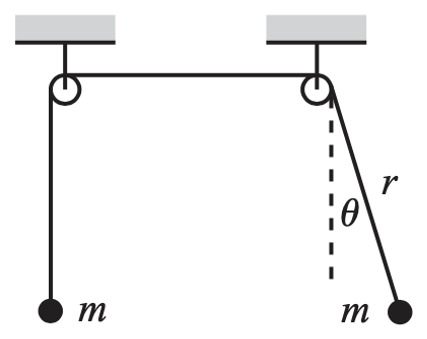
\includegraphics[width=0.4\textwidth]{Finala_P9.png}
%     \label{P7}
% \end{figure}


\end{document}